%%% Realisering af optimering af current-sense filter %%%

\subsection{Current-sense filter}
For at teste optimeringen af current-sense filteret, måles signalet både før og efter filteret. Det filtrerede signal ses på figur~\ref{fig:Realisering_cs_M_3}, hvor kanal 1 viser current-sense signalet, og kanal 2 viser MOSFET'ens gate. Det viser, at der opnået et filter med stort set rette flanker, og dermed en meget hurtigere stigetid. Figur~\ref{fig:Realisering_cs_M_zoom_3} viser current-sense signalet, hvor der er zoomet ind på flanken. Her aflæses stigetiden til ca. $100ns$. Samtidig ses det lille overshoot, som også kom ved simuleringen. Det viser, der er opnået en optimal stigetid i filteret. Resultaterne for analyse, simulering og realisering er indført i tabel~\ref{label}.

\begin{table}[H] 			
	\centering
	\begin{tabularx}{\textwidth}{|X|c|c|c|}
		\hline
		\textbf{Tid} & \multicolumn{3}{|c|}{\textbf{Switch-tid}} 										\\ \hline
		& A & S & R 									\\ \hline
		$T_{r}$ & $100ns$ & $85ns$ & $100ns$ 										\\ \hline 
	\end{tabularx}
	\caption{Resultater for analyse, simulering og realisering af current-sense filter}
	\label{tab:resultat_cs_filter_3}
\end{table}


\begin{figure}[H]
	\center
	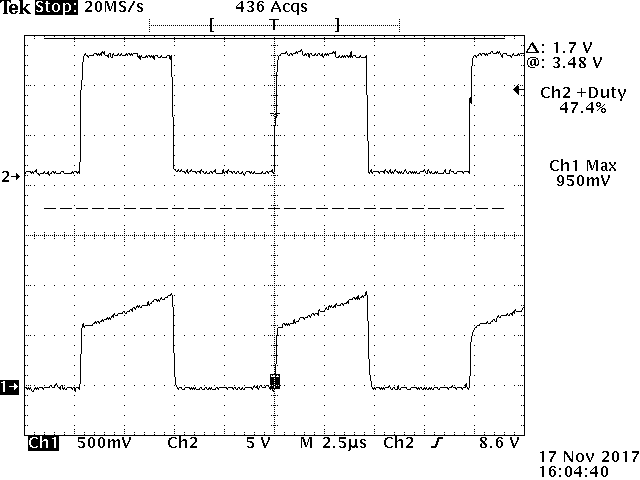
\includegraphics[max width=0.7\linewidth]{/tex/3iteration/billeder/Realisering/Realisering_cs_M.png}
	\caption{Realisering af optimering af current-sense signal efter filtrering}
	\label{fig:Realisering_cs_M_3}
\end{figure}

\begin{figure}[H]
	\center
	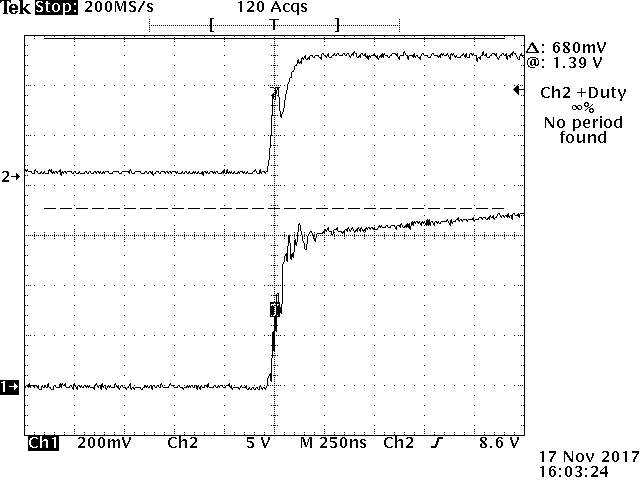
\includegraphics[max width=0.7\linewidth]{/tex/3iteration/billeder/Realisering/Realisering_cs_M_zoom.png}
	\caption{Realisering af optimering af current-sense signal efter filtrering - zoom}
	\label{fig:Realisering_cs_M_zoom_3}
\end{figure}